\documentclass[12pt,fleqn]{article}\usepackage{../../common}
\begin{document}
Ders 29

[onceki ders tekrari atlandi]

Uzaklaşım teorisinin ispatına gelelim. Bu ispatın daha kolay versiyonunu
yapacağım şimdi, tüm eşitlik yerine

$$
\int \oint_S < 0,0,R > \cdot \hat{n} \ud S =
\iiint_D R_z \ud V
$$

eşitliğinin ispatını yapacağım. Buradan hareketle daha genel eşitliği
ispatlamak kolay, aynı ispatı sadece $x$, sadece $y$ bileşeni olan
vektör alanları için tekrarlarım, ve tüm bunları toplayınca ana eşitliği
elde etmiş olurum.

İkinci bir basitleştirme yapalım, çünkü ispatı hala herhangi bir yüzey için
yapabileceğimden emin değilim. Dikey, basit bir yüzey kullanacağım, öyle ki
bu yüzey üzerinden entegralde $z$ değişkenin sınırlarını kolay halledebileyim.

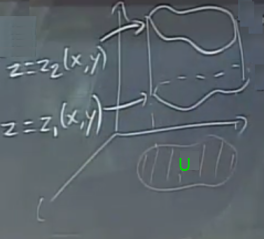
\includegraphics[width=15em]{calc_multi_29_01.png}

Bir üst yüzey var bir alt var, aralarında kalan yüzey dikey. Burada kullandığım
kavram, dikey basit bölge (vertically simple region) iki yüzey arasındaki bölge.

Başlayalım, üstteki formülün sağ ta rafındaki entegrali hesaplayalım. Bu
hesaptan bir sayı çıkmayacak tabii ki çünkü pek çok şeyi tanımsız bıraktık, ama
en azından bazı basitleştirmeler yapabiliriz, mesela bir ölçüde $z$ üzerinden
entegral alabilirim. 

$$
\iiint_D R_z \ud V = \iint \int_?^? R_z \ud z \ud x \ud y
$$

$z$'nin sınırları nedir? Hatırlarsak üçlü entegralde $z$ üzerinden entegral
alırken ise $x,y$ değişkenlerini sabitleyerek başlıyorduk, ve o sabitlenen
$x,y$'den yukarı çıkıp bir dikey kesite bakıyorduk ve sınırların nereye
geldiğini not ediyorduk. Üstteki bölge için bu altta $z_1$, üstte $z_2$. 

$$
= \iint \int_{z_1}^{z_2} R_z \ud z \ud x \ud y
$$

Şimdi tüm mümkün $x,y$ için entegralin geri kalanını hesaplamak istiyorum,
bu üstteki dikey bölgenin gölgesindeki alan $U$ içinde olacak, 

$$
= \iint_U \left( \int_{z_1(x,y)}^{z_2(x,y)} R_z \ud z  \right) \ud x \ud y  
$$

Üstteki entegrali hesaplamayı düşünürsek, en içteki entegral fazla kötü durmuyor
aslında, $R$'nin $z$'ye göre türevi var, sonra $z$ üzerinden entegral alınıyor.
Bu bize $R$'yi geri vermez mi? Evet. O zaman

$$
\iiint_D R_z \ud V = \iint_U \bigg[ R(x,y,z_2(x,y)) - R(x,y,z_1(x,y))  \bigg]
\ud x \ud y
$$

Elde net formül olmadan daha fazla ilerleyemem, şimdi çift entegrale dönüyorum.
Bu entegralde $S$ var, ve $S$ alt, üst ve yan yüzeylerden oluşan kapalı bölge.

$$
\int \oint_{S = \textrm{alt+üst+kenarlar}} < 0,0,R > \cdot \hat{n} \ud S =
\iint_{\textrm{üst}} + \iint_{\textrm{alt}} + \iint_{\textrm{kenarlar}} 
$$

Üst yüzey ile başlayalım. Akış entegralindeki $\hat{n} \ud S$'i o yüzey
için hazırlamak lazım. İyi haber üst, alt yüzeyin $x,y$ üzerinden bir $z$
formülü var, ve bu tür formül olunca $\hat{n} \ud S$'i nasıl hesaplayacağımızı
biliyoruz, mesela $z=z_2(x,y)$ için,

$$
\hat{n} \ud S = <
-\frac{\partial z_2}{\partial x}, 
-\frac{\partial z_2}{\partial y},
1
> \ud x \ud y
$$












[devam edecek]

\end{document}
